\documentclass[12pt,a4paper]{article}

\usepackage[utf8]{inputenc}
\usepackage{amsmath}
\usepackage{amsfonts}
\usepackage{amssymb}
\usepackage{graphicx}
\usepackage[margin=0.5in]{geometry}

\graphicspath{{./images/}}
\author{Oleg Loshkin}
\title{\textbf{UPDC}\\Unity to PokEngine Data Converter\\\textbf{Technical Document}}

\begin{document}

\maketitle
\section{Introduction}
	\begin{itemize}
		\item \textbf{Project's Context}
		\\As part of the game programming cursus at SAE Institute Geneva, for the \textbf{technical module GPR5100.2}, students of the second year must \textbf{assist students from the third year in completing their bachelor’s project.}\\\\
		This year, the third year's \textbf{PokFamily team} develops a \textbf{video game for the Switch} and PC using a tailored \textbf{in-house engine}.\\Second year students must \textbf{assist them} by creating various \textbf{tools they will need} in order to create their game.\\\\
		This document describes the functioning of the \textbf{Unity to PokEngine Data Converter} tool, \textbf{UPDC} for short.
		
		\item \textbf{Project's Goals}
			\begin{itemize}
				\item Create a useful tool that the PokFamily team will use to create their video game.
				
				\item Learn to work in a non-academic environment in a team that depends on the student’s performance.
				
			\end{itemize}
			
		\item \textbf{Specific Problem}
		\\The PokFamily team uses the \textbf{Unity engine as an external editor}. The PokFamily team needs a tool to \textbf{convert ScriptableObjects to a JSON} format \textbf{readable by the PokEngine} parser. This tool may then be used by other Unity tools to export data.
	\end{itemize}
\newpage

\section{Requirements}
This project’s requirements have two origins:
\begin{itemize}
	\item \textbf{Academic requirements}
		\begin{itemize}
			\item The task given by the team has been understood and done in time.
			
			\item The tool is maintained by the student after the tool's completion.
			
			\item The tool must be user-friendly.
			
			\item The student understands how to manage data.
			
			\item The student understands how a game engine interfaces with a game engine editor.
			
			\item The student has organized himself and his work in a way to facilitate the work of others.
			
			\item The tool’s performance is reasonable.
			
			\item The implementation is appropriately sophisticated.
			
			\item The student understands the implications of non-academic teamwork.
			
		\end{itemize}
	\item \textbf{Pragmatic requirements}
		\begin{itemize}
			\item Convert ScriptableObject files to files readable by the PokEngine's parser.
			
			\item The user must be able to interact with the tool via Unity.
			
			\item The code must satisfy the quality and style expected by the team. C++ coding style is defined in the Coding Style Document. C\# coding style is defined in UnityWorkOrganization document.
			
			\item The student must communicate with the team appropriately and be dependable.
			
			\item Allow other tools to export data via the UPDC.
			
	\end{itemize}
\end{itemize}
\newpage

\section{Technologies Used}
\begin{itemize}
	\item \textbf{PokEngine}\\
		The \textbf{PokEngine} is the game engine developed by the PokFamily team. The engine is \textbf{written with C++ standard 2014} and \textbf{partly C++ standard 2014} for code running on the Nintendo Switch.\\
The engine has a parser that is capable of reading JSON files. This parser is used to import data exported from Unity with UPDC.

	\item \textbf{Unity 2019.1.10f}\\
		Unity 2019.1.10f is used as an \textbf{external editor}.
	
	\item \textbf{Visual Studio 2017}\\
		Visual Studio 2017 is used for development of the PokEngine.
	
	\item \textbf{Git}\\
		\textbf{github.com} is used for versioning for the \textbf{PokEngine source code}. \textbf{gitlab.com} is used for versioning for the \textbf{Unity prototype source code}. Git bash is used for most interactions with the git framework. Merge conflicts are solved manually via text editor and git bash.
		
\end{itemize}

\section{Interaction with Overall Project}
\begin{center}
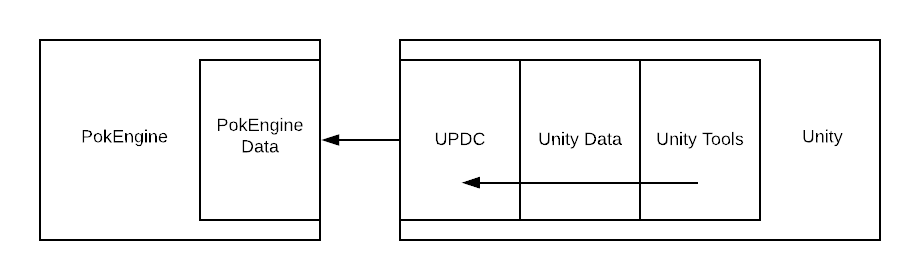
\includegraphics[scale=0.5]{UPDCLocation}
\end{center}
UPDC provides other Unity tools to export data to be used by the PokEngine. As such, it is the last chain link that's still part of Unity before said data leaves Unity altogether to integrate the PokEngine side of the project.

\section{UML Diagram}
\begin{center}
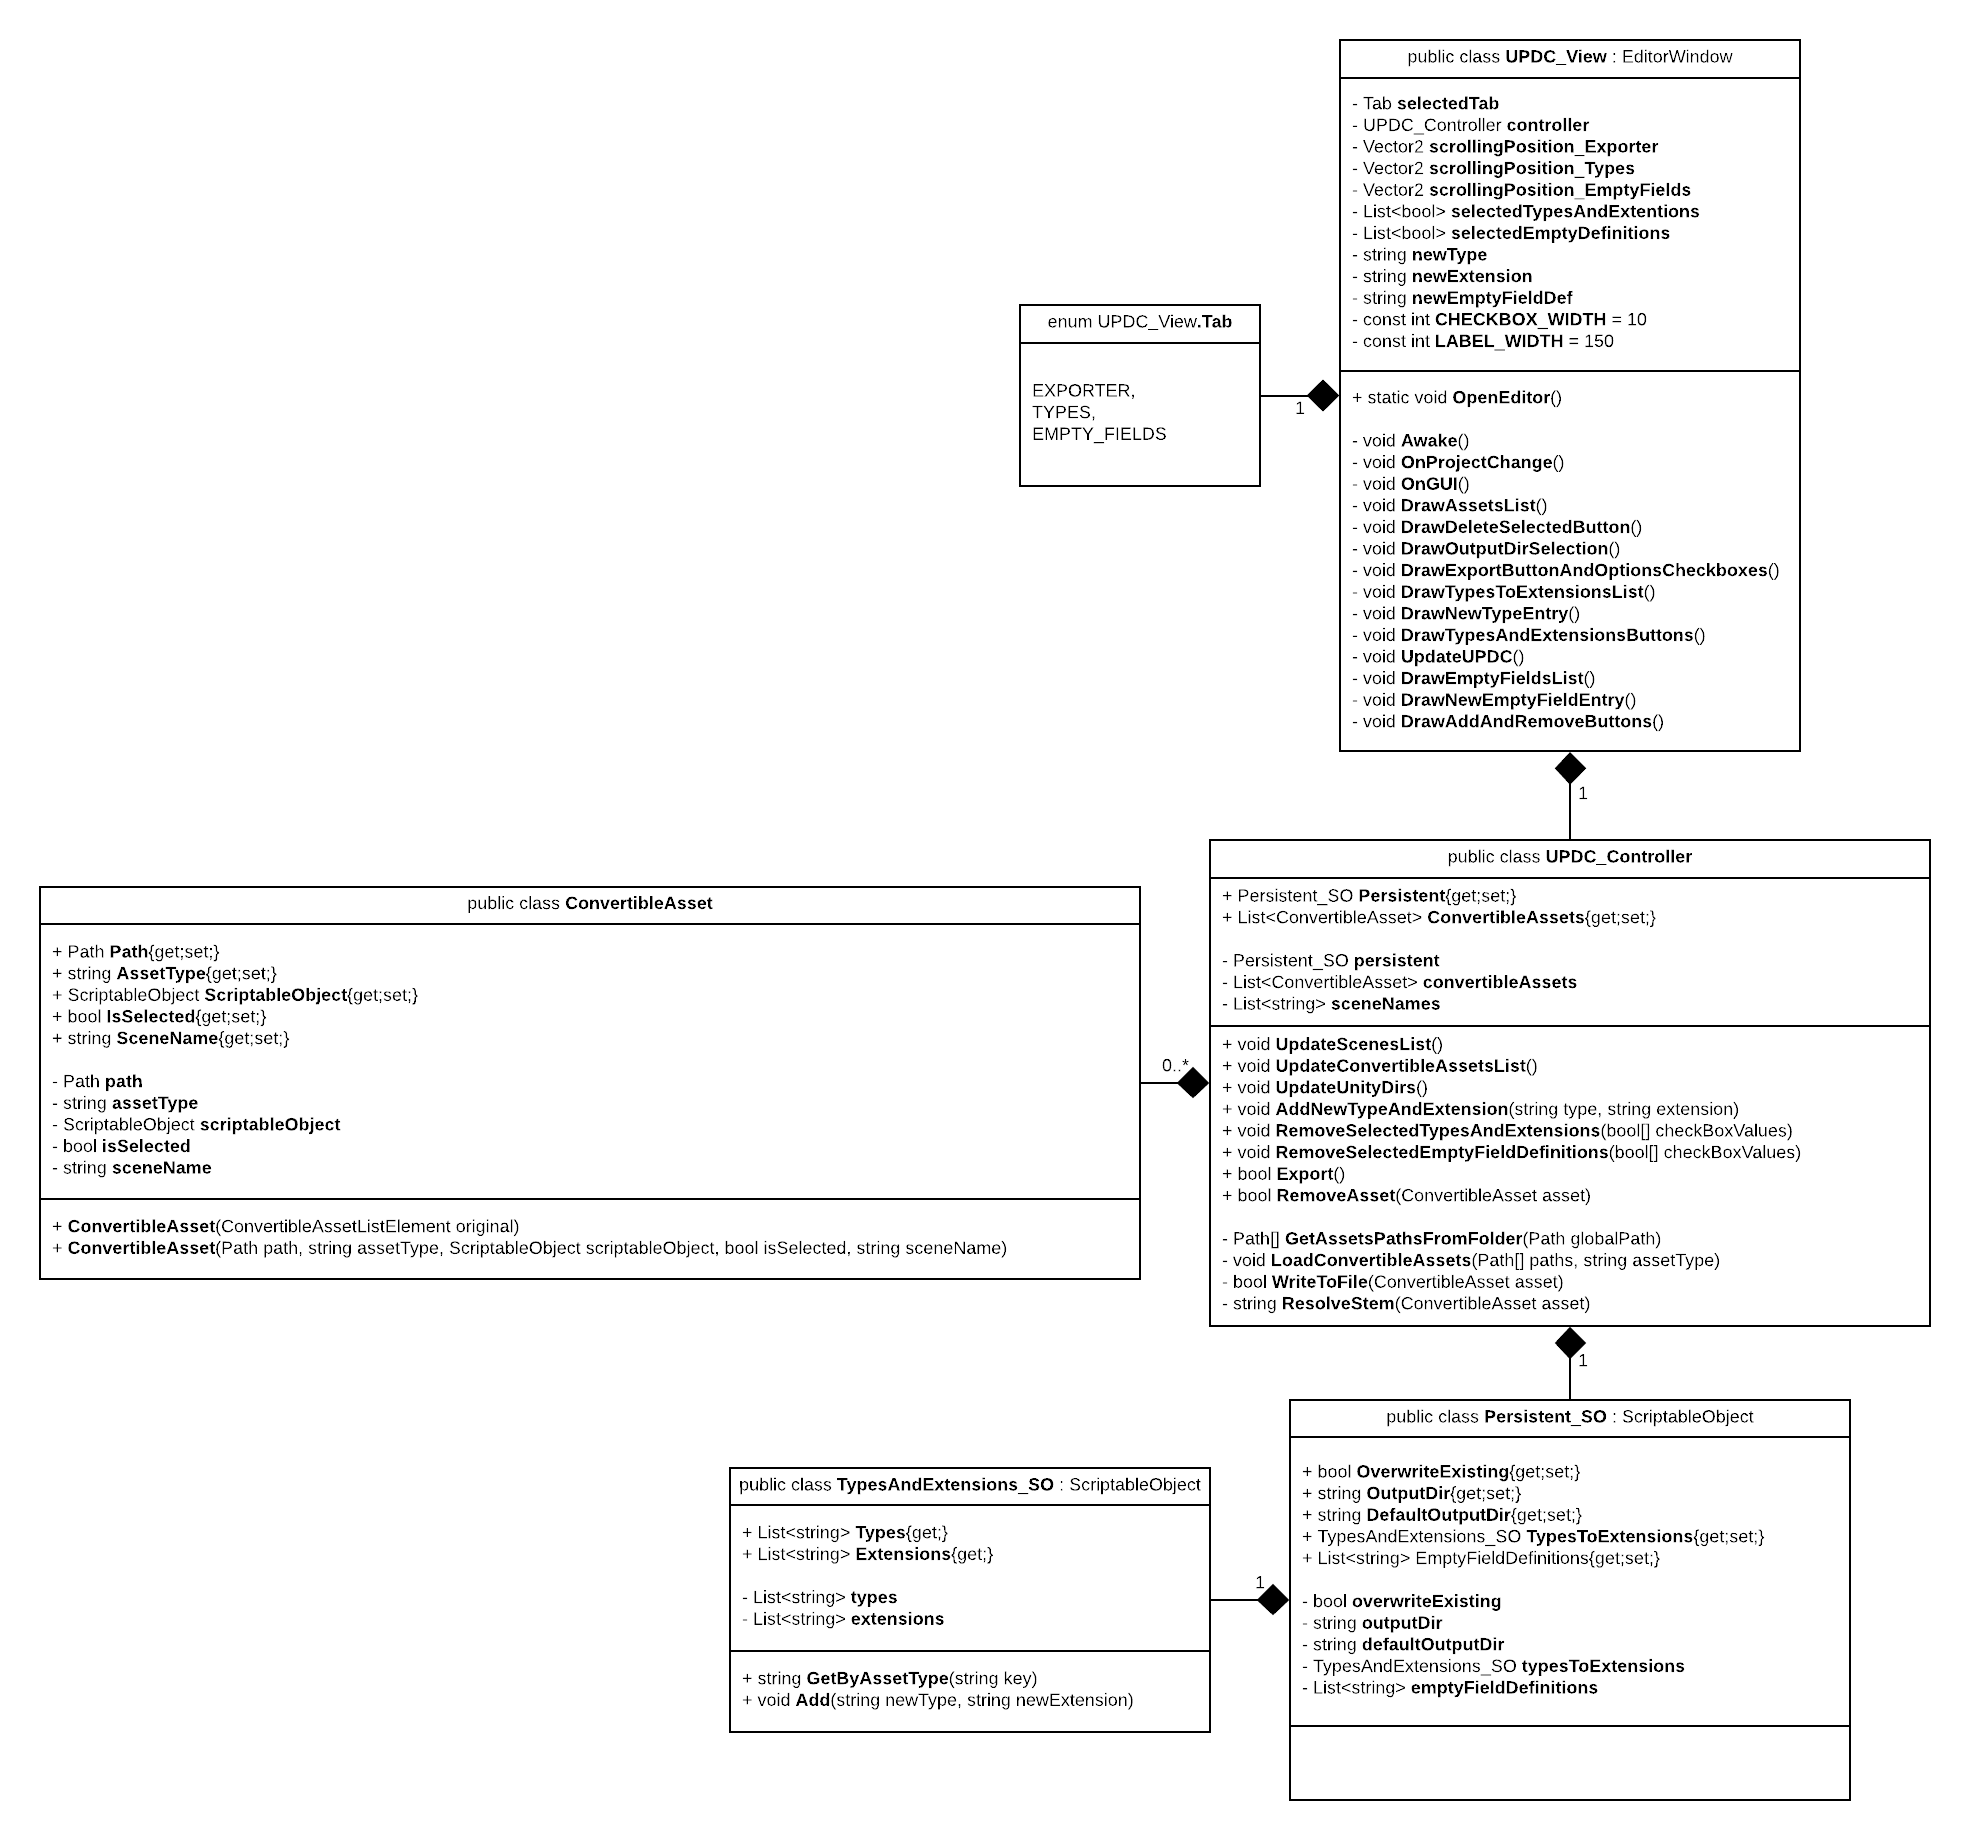
\includegraphics[scale=0.25]{UMLUPDC}
\end{center}
\noindent The tool follows a \textbf{Model-View-Controller} model where the model is Unity's data, the view is \texttt{UPDC\_View} and the controller is \texttt{UPDC\_Controller}.\\
\textbf{ScriptableObjects are used to store user data across sessions}. Said data includes:
\begin{itemize}
\item Whether or not to overwrite any existing files upon export.
\item Whether or not to export the JSON data in a format easily readable by humans, or to prefer optimisation.
\item Last selected output directory for export.
\item Default output directory for export.
\item A dictionary like class to keep track of defined types and extensions managed by the UPDC.
\end{itemize}
\newpage

\section{Tackling Genericity}
\textbf{UPDC needs to be able to export} various data types that \textbf{aren't well defined in advance}. With project advancement, new types of data may need to be exported besides the ones currently developed by the team. This means that \textbf{the implementation of the tool had to be flexible and not hard-coded}.\\\\
The \textbf{tool addresses this constraint by making use of Unity's ScriptableObject class}. ScriptableObjects are Unity's way of handling persistent data and the engine has well developed functionalities for manipulating ScriptableObjects. JSONUtility was used for generating JSON files from ScriptableObject objects for instance. This did however come with the drawback of not being able to ignore empty fields, that are currently written to the JSON file when it would have been preferable to remove these altogether.\\\\
\textbf{By using a string to string dictionary} like class (\texttt{TypesAndExtensions\_SO}), UPDC allows to \textbf{add and remove support any new convertible asset types without requiring the user to interact with UPDC's code} provided the type defined inherits from the ScriptableObject class.

\section{Working with JSONUtility}
\textbf{Unity's JSONUtility helper class was used to convert ScriptableObjects into JSON formatted strings} that were then written to disk. Using it meant that \textbf{no custom parser needed to be implemented for this tool, however there were drawbacks in using it later down the line.}\\\\
\textbf{Unity's serialization system considers every object like a struct type}, meaning that any serialized data structure, be it a class or a struct, is \textbf{written down in full in the output JSON string}, including default values for any uninitialized fields of the object being serialized. This leads to the \textbf{JSON string getting bloated with unnecessary data}.\\\\
\textbf{To prevent this problem, an additional parsing pass was added} on UPDC's side to \textbf{remove any uninitialized fields} from the JSON string provided by JSONUtility before being written down to file.
\begin{center}
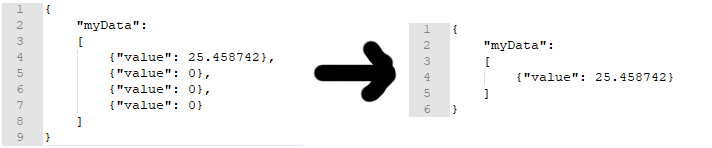
\includegraphics[scale=1.0]{cleaningJson}
\end{center}

\section{Tool's UI}
\begin{center}
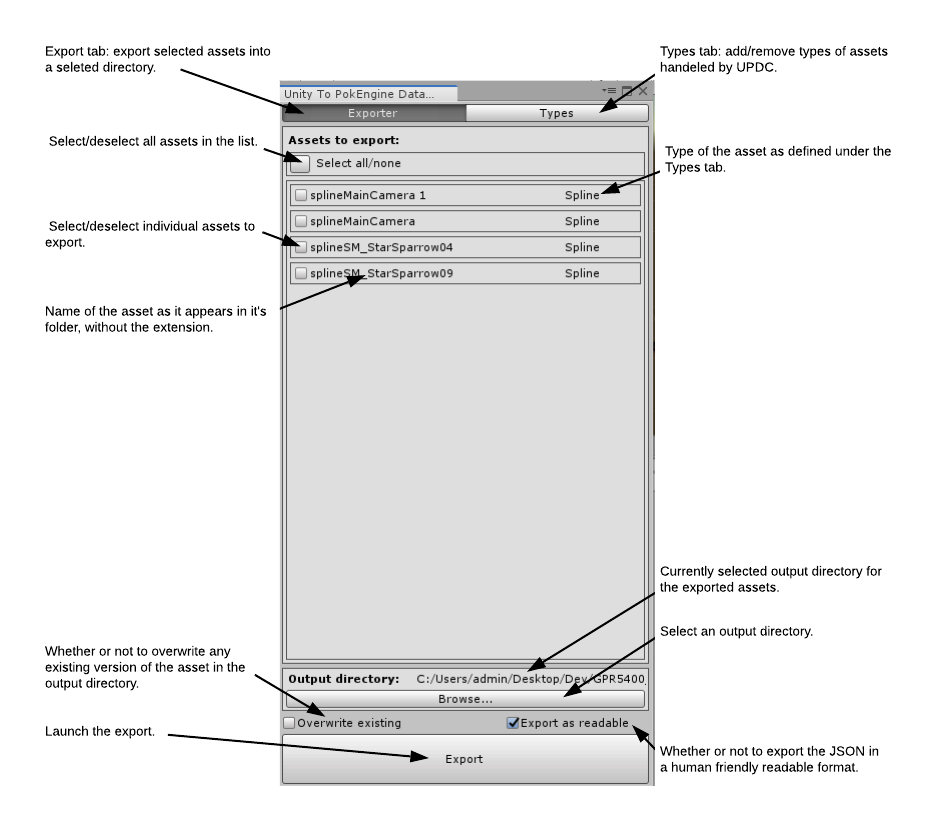
\includegraphics[scale=0.5]{exportUi}
\end{center}
\begin{center}
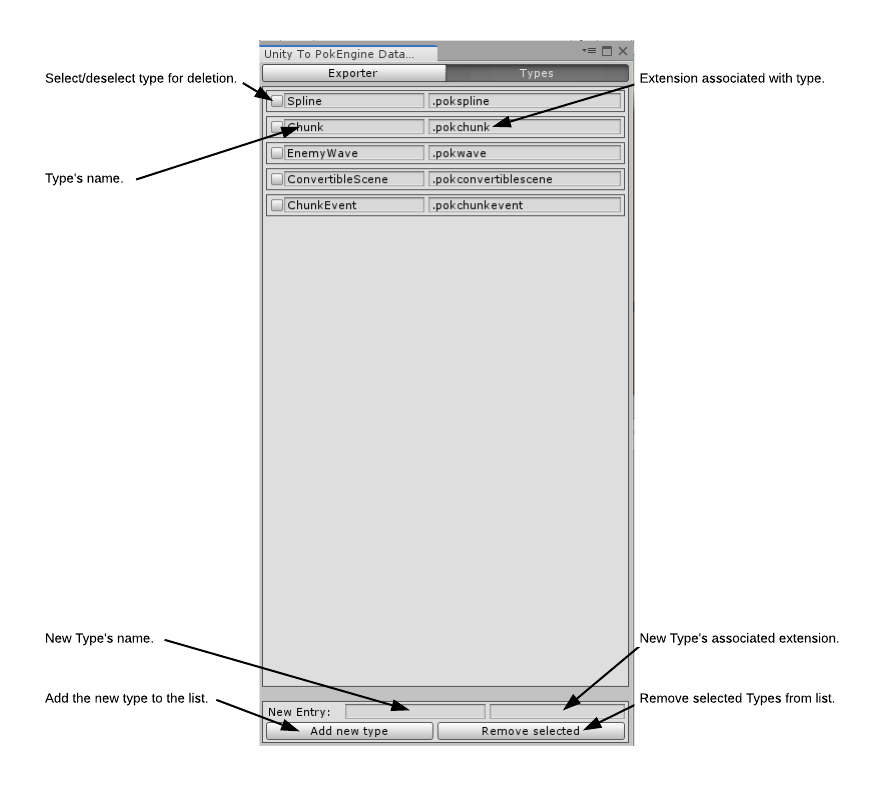
\includegraphics[scale=0.6]{typesUi}
\end{center}
\begin{center}
\includegraphics[scale=0.6]{emptyfieldsui}
\end{center}
\newpage

\section{Potential Improvements}
\begin{itemize}
\item Implementation of an new convertible type still requires the user to create their data structure and store the ScriptableObject instances in the correct folder on their own. It would have been better to provide an automated way to do so.
\end{itemize}

\section{Summary}
\textbf{The UPDC tool allows other Unity tools to export Unity data into JSON files} readable by the PokEngine parser and \textbf{it's implementation is flexible enough to quickly integrate new data types}.\\\\

\end{document}